% Section: Overview of the project
\section{Overview of the project}
\label{sec:overview}

\subsection{Organisation in folders}
\label{sec:folders}

The C++ sources of \CAP{} are in \code{src}, in four folders, each holding one library per sub-folder, built as a
shared library of the same name (Table~\ref{tab:libraries}).

\paragraph{\code{src/core}.}
The core holds what does not depend on particles or events: Base (objects, folders, reflection, tasks, configuration,
XML and binary files; Section~\ref{sec:base}), Math (data, functions, fits and the other numerical classes;
Section~\ref{sec:math}), Graphics, Latex and Interpreter (figures, documents and the command language;
Section~\ref{sec:graphics}), and Helpers, which converts histograms between ROOT files and CAP files. The core is
usable on its own, for work that has nothing to do with collisions: fitting data, drawing them, or storing them.

\paragraph{\code{src/analysis}.}
The analyses hold the event processing: the library Particles, the framework shared by all analyses (events,
particles, particle databases, filters, efficiencies, smearers, the base classes of the analysis tasks and of their
histogram folders; Section~\ref{sec:analysis}), and one library per family of observables (Section~\ref{sec:observables}):
single-particle spectra (ParticleSingle), pair correlations (ParticlePair) and their three-dimensional version
(ParticlePair3D), transverse-momentum correlators (PtPt), multiplicity fluctuations (NuDyn), anisotropic flow
(ParticleFlow), global observables (Global) and event shapes (Spherocity), performance studies (Performance), the
combination of sub-samples (SubSample), and jet analyses (Jets, optional).

\paragraph{\code{src/models}.}
The models produce events (Section~\ref{sec:generators}): a simple generator (BasicEventGen), the Glauber model of
nucleus--nucleus collisions (Glauber), a thermal model (Therminator3), interfaces to Pythia~8 and Herwig~7 (Pythia,
Herwig, optional), and readers of the events of EPOS and PHSD (Epos, PHSD).

\paragraph{\code{src/gui}.}
The sources of the graphical interface CapGui (Section~\ref{sec:capgui}).

\paragraph{Other folders.}
The top-level folder of \CAP{} also holds the Python front ends (\code{BuildCAP.py}, \code{RunCAP.py} and the
particle-database editor \code{ParticleDbEditor.py}) and the script \code{SetupCAP.sh}, which sets the environment
variables of \CAP{}; \code{DB}, the data that jobs read: the particle database (\code{DB/ParticleData}, an XML file
of the particles and their decay modes), the inputs of the thermal model (\code{DB/Therminator}), and the XML
templates of the task classes (\code{DB/Templates}, Section~\ref{sec:xml}); \code{projects}, example workflows of
the generators (Pythia, Therminator, Glauber, PHSD, and a Gaussian test); \code{external}, the sources of the
libraries distributed with \CAP{} for CapGui (Dear ImGui, GLFW, NanoSVG); \code{Grid}, scripts submitting jobs to
the computing clusters of the authors; \code{tests}, the tests of the Python front ends; and \code{docs}.
The libraries and the programs are installed in \code{lib} and \code{bin}.

\begin{table}[t]
  \centering
  \caption{Libraries of \CAP{}, with the libraries of \CAP{} they link to (those reached through them are not
  repeated) and the size of their sources, in thousands of lines, tests excluded. Optional libraries are marked with
  an asterisk.}
  \label{tab:libraries}
  \small
  \begin{tabular}{@{}p{5cm}llr@{}}
    \toprule
    Library & Folder & Uses & kLines \\
    \midrule
    Base           & core     & ---                                & 21.1 \\
    Math           & core     & Base                               & 39.3 \\
    Helpers        & core     & Math; ROOT                         &  7.3 \\
    Graphics$^*$   & core     & Math; LaTeX (optional)             & 11.6 \\
    Latex$^*$      & core     & Helpers, Graphics                  &  1.8 \\
    Interpreter    & core     & Math; Graphics, Latex (if built)   &  1.9 \\
    \midrule
    Particles      & analysis & Helpers                            & 13.6 \\
    \raggedright ParticleSingle, PtPt, NuDyn, Global, Spherocity & analysis & Particles & 4.6 \\
    ParticleFlow   & analysis & Particles                          &  1.6 \\
    ParticlePair, ParticlePair3D & analysis & ParticleSingle      &  6.7 \\
    Performance, SubSample & analysis & Particles                 &  3.1 \\
    Jets$^*$       & analysis & Particles; FastJet                 &  1.3 \\
    \midrule
    \raggedright BasicEventGen, Epos$^*$, PHSD$^*$ & models & Particles         &  0.7 \\
    Glauber        & models   & Particles                          &  9.3 \\
    Therminator3$^*$ & models & Particles                          &  4.8 \\
    Pythia$^*$     & models   & Particles; Pythia8                 &  0.8 \\
    Herwig$^*$     & models   & Particles; Herwig, ThePEG          &  0.5 \\
    \midrule
    CapGui$^*$ (program) & gui & Graphics; Dear ImGui, GLFW, OpenGL &  9.4 \\
    \bottomrule
  \end{tabular}
\end{table}

% ---------------------------------------------------------------------------------------------------------------
\subsection{Layers and dependencies}
\label{sec:layers}

The libraries form layers (Fig.~\ref{fig:layers}), each of which uses only the layers below it. Base depends on no
other library of \CAP{}, and Math only on Base. Graphics, Latex and Interpreter use Math but no part of the analyses,
so that the figures, documents and scripts work on any data. The framework of the analyses, Particles, uses the core;
the analyses and the models use Particles, and never each other, with one exception: the pair analyses use the
single-particle histograms of ParticleSingle. The models and the analyses therefore meet only through the events
and the tasks of Particles: a new generator works with every analysis, and a new analysis with every generator.

Four programs sit on top. \code{CAP} runs the jobs: it links the analyses and the models, so that every task class
they register can be named in a workflow, and creates the tasks of a job by name through the registry of classes
(Section~\ref{sec:objects}). CapShell runs the command language of Interpreter. CapGui shows and fits the content of
CAP files (Section~\ref{sec:capgui}); it uses the core only, so that it reads the results of every analysis without
linking any of them, since the files hold histograms and folders of the core. \code{CapRootConvert} converts
histograms between ROOT and CAP files. The Python front ends are not linked to anything: \code{BuildCAP.py} runs
CMake, and \code{RunCAP.py} writes workflow files and runs \code{CAP} on them.

\begin{figure}[t]
  \centering
  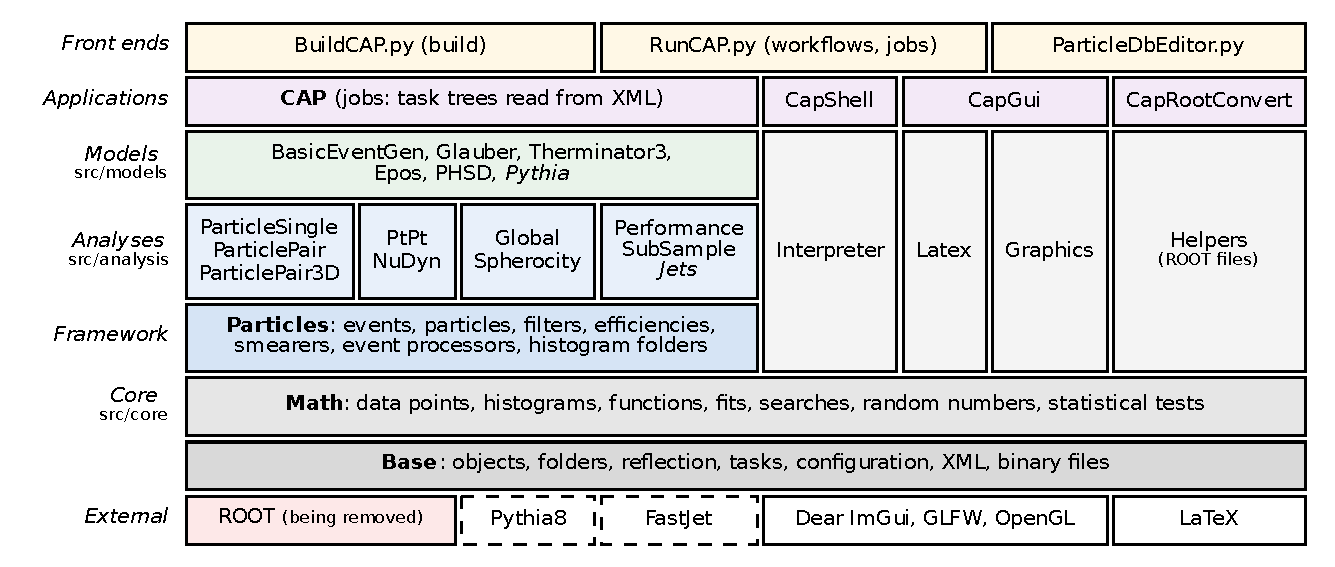
\includegraphics[width=\textwidth]{Layers}
  \caption{Layers of \CAP{}. Each layer uses only the layers below it; the libraries of the core on the right
  (Interpreter, Latex, Graphics, Helpers) use Math and Base, and not the analyses. Names in italics are optional
  modules; dashed boxes are optional external packages. The uses of ROOT that remain in the core and in the analyses are
  being removed (Section~\ref{sec:external}).}
  \label{fig:layers}
\end{figure}

% ---------------------------------------------------------------------------------------------------------------
\subsection{External software}
\label{sec:external}

\paragraph{Required.}
\CAP{} is built with CMake (3.5 or later) and a C++17 compiler; it is developed on macOS with Clang and built on Linux
with GCC. ROOT~\cite{Brun:1997pa} is still required to build it. Its remaining uses are listed here, as they are
the work left to make \CAP{} independent of ROOT: random numbers (\code{gRandom}) in a few tasks of the analyses and
models; system utilities and the \code{TString} class used by older code in Base; the reading of ROOT files by some
tasks; and the Glauber and Therminator3 models, written for earlier versions of \CAP{}. The conversion of
histograms from and to ROOT files (Helpers, \code{CapRootConvert}, and the reading of ROOT files by CapGui) will keep
using ROOT, but as an option (\code{CAP\_WITH\_ROOT\_FILES}). The front ends need Python~3.7 or later with tkinter.
\todo{\code{src/CMakeLists.txt} sets \code{CMAKE\_CXX\_STANDARD} to 14; the code is compiled as C++17 only because
the flags of ROOT ask for it. Set the standard to 17 before submission.}

\paragraph{Optional.}
The interfaces to Pythia~8~\cite{Bierlich:2022pfr} and Herwig~7~\cite{Bellm:2015jjp}, and the jet analyses, which
use FastJet~\cite{Cacciari:2011ma}, are built when asked for. CMake looks for each package in turn in a copy
distributed with \CAP{} (a folder \code{pythia8*}, \code{Herwig*} or \code{fastjet*} in the \CAP{} folder or in
\code{external}, or an installation \code{../Herwig/install} or \code{../Fastjet/install} next to the \CAP{} folder),
at the location given by an environment variable, and through the configuration tool of the package
(\code{pythia8-config}, \code{Herwig-config}, \code{fastjet-config}), or uses the location given explicitly. A LaTeX installation with \code{dvisvgm} is used, when
present, to typeset the texts of the figures (Section~\ref{sec:graphicscore}), and \code{pdflatex} to compile the
presentations; without them, texts are drawn with plain fonts. CapShell uses the \code{editline} library, when
present, for line editing and history.

\paragraph{Distributed with \CAP{}.}
CapGui is built on Dear ImGui~\cite{DearImGui} and GLFW, whose sources are in \code{external} and are compiled with
\CAP{}, and on OpenGL, which every desktop system provides; the texts typeset by LaTeX are rasterised for the screen with NanoSVG. Nothing else needs to be
installed to build the interface.

% ---------------------------------------------------------------------------------------------------------------
\subsection{Building: BuildCAP.py}
\label{sec:build}

\CAP{} is built with CMake, in a build folder of the \CAP{} folder, and installed in its folders \code{lib} and
\code{bin}. The script \code{BuildCAP.py} is a window from which the build is configured and run (Fig.~\todo{screenshot}).
It lists the core modules, always built, and the optional modules (Therminator3, Latex, Graphics, CapGui, the
conversion of ROOT files, Jets, Epos, PHSD, Pythia and Herwig), each with a check box, together with the locations of ROOT and of
the external packages; a button shows which installation of each package CMake will use. A toolbar chooses the build
folder, the build type, the number of parallel jobs, and whether to install, and the output of CMake and make is shown
in the lower half of the window and can be saved. Each command is printed before it runs, and the same build is made
from a terminal with
\begin{verbatim}
source SetupCAP.sh
cmake -S src -B build -DCAP_WITH_PYTHIA8=ON -DCAP_PYTHIA8_DIR=/opt/pythia8   # options as needed
make -C build -j8 install
\end{verbatim}
\code{BuildCAP.py -{}-print-commands} prints the commands of the saved settings without opening the window. Several build
folders can coexist, for instance one with Pythia and one without, or a release and a debug build. The environment
of \code{SetupCAP.sh} (the paths of \CAP{}, its libraries, its programs, its database and its projects) is set for the
commands, verbatim that the window works without a prepared shell. After a build, \code{ctest} runs the tests of the
modules: the test programs of Base, Math, Graphics, Latex, Interpreter, Helpers and Therminator3, and the tests of
the Python front ends.

% ---------------------------------------------------------------------------------------------------------------
\subsection{Running: RunCAP.py}
\label{sec:run}

\paragraph{Workflows.}
An analysis is described by a workflow file (Section~\ref{sec:xml}), which \code{RunCAP.py} composes, checks and
runs (Fig.~\todo{screenshot}). Its window has four parts. The workflow editor lists, on the left, the task classes of
the current build, read from their XML templates (which are regenerated when the program or the libraries are newer
than them), and on the right the tasks of the workflow; tasks are added, removed, ordered and nested, a nested task
being a subtask of the task above it, such as a generator and the analyzers inside an event iterator. A task can be
added several times, each copy with its own parameters. The filter editor defines the event and particle filters, the
efficiencies and the smearers of the workflow once, by their conditions or their parameters; they are created at the
start of the job by a filter-creator task, and each task chooses those it uses by name (Section~\ref{sec:filters}).
The task list shows, for each task in the order of execution, the filters it uses, its number of histogram folders,
and the first problem found in its configuration. A double click opens the window of a task, with its general
settings (name, report level, filters, efficiencies, particle databases, parameters) and its histograms: for each list
of folders, whether it is used, created, imported or exported, the prefix of the names of the folders, and either one
binning for all the folders or a binning per folder. The fields check the type of the values they accept. The values
read from a workflow file are checked against the templates, so that a misspelled or obsolete parameter is reported
when the file is loaded.

\paragraph{Stages and jobs.}
A workflow has up to three stages, which are the phases of Section~\ref{sec:phases}: event processing, derived
histograms and balance functions. Each stage is run as a job of its own,
\begin{verbatim}
bin/CAP <stage task> <directory of the workflow>/ <workflow file> <output directory>/
\end{verbatim}
the stages running one after the other, each reading the output file of the previous one. The derived-histogram stage is
made by \code{RunCAP.py} from the analyzers of the first stage, the first time it is shown: each analyzer gets its
calculator, with the same filters and histogram settings, so that the folders of the two jobs match. The output of
\CAP{} is shown as it runs, can be saved, and a job can be stopped. The same workflow file is run without the
window, on a cluster for instance, with the command above, which \code{RunCAP.py -{}-print-command} prints;
\code{RunCAP.py -{}-check} checks a file against the templates.
\todo{the scripts of \code{Grid} that submit many jobs and combine their outputs (Section~\ref{sec:subsample}).}
